\documentclass[a4paper]{article}\usepackage[]{graphicx}\usepackage[]{color}
%% maxwidth is the original width if it is less than linewidth
%% otherwise use linewidth (to make sure the graphics do not exceed the margin)
\makeatletter
\def\maxwidth{ %
  \ifdim\Gin@nat@width>\linewidth
    \linewidth
  \else
    \Gin@nat@width
  \fi
}
\makeatother

\definecolor{fgcolor}{rgb}{0.345, 0.345, 0.345}
\newcommand{\hlnum}[1]{\textcolor[rgb]{0.686,0.059,0.569}{#1}}%
\newcommand{\hlstr}[1]{\textcolor[rgb]{0.192,0.494,0.8}{#1}}%
\newcommand{\hlcom}[1]{\textcolor[rgb]{0.678,0.584,0.686}{\textit{#1}}}%
\newcommand{\hlopt}[1]{\textcolor[rgb]{0,0,0}{#1}}%
\newcommand{\hlstd}[1]{\textcolor[rgb]{0.345,0.345,0.345}{#1}}%
\newcommand{\hlkwa}[1]{\textcolor[rgb]{0.161,0.373,0.58}{\textbf{#1}}}%
\newcommand{\hlkwb}[1]{\textcolor[rgb]{0.69,0.353,0.396}{#1}}%
\newcommand{\hlkwc}[1]{\textcolor[rgb]{0.333,0.667,0.333}{#1}}%
\newcommand{\hlkwd}[1]{\textcolor[rgb]{0.737,0.353,0.396}{\textbf{#1}}}%
\let\hlipl\hlkwb

\usepackage{framed}
\makeatletter
\newenvironment{kframe}{%
 \def\at@end@of@kframe{}%
 \ifinner\ifhmode%
  \def\at@end@of@kframe{\end{minipage}}%
  \begin{minipage}{\columnwidth}%
 \fi\fi%
 \def\FrameCommand##1{\hskip\@totalleftmargin \hskip-\fboxsep
 \colorbox{shadecolor}{##1}\hskip-\fboxsep
     % There is no \\@totalrightmargin, so:
     \hskip-\linewidth \hskip-\@totalleftmargin \hskip\columnwidth}%
 \MakeFramed {\advance\hsize-\width
   \@totalleftmargin\z@ \linewidth\hsize
   \@setminipage}}%
 {\par\unskip\endMakeFramed%
 \at@end@of@kframe}
\makeatother

\definecolor{shadecolor}{rgb}{.97, .97, .97}
\definecolor{messagecolor}{rgb}{0, 0, 0}
\definecolor{warningcolor}{rgb}{1, 0, 1}
\definecolor{errorcolor}{rgb}{1, 0, 0}
\newenvironment{knitrout}{}{} % an empty environment to be redefined in TeX

\usepackage{alltt}
\usepackage{a4wide}
\usepackage[margin=.8in]{geometry}
\usepackage{colortbl}

\title{Comparison of Versions of Kinship Links}
\author{Joe Rodger's BG Team}
\IfFileExists{upquote.sty}{\usepackage{upquote}}{}
\begin{document}

\maketitle

\definecolor{goodColor}{rgb}{.9,1,.85}
\definecolor{sosoColor}{rgb}{1,0.9215686,0.6117647}
\definecolor{badColor}{rgb}{1,.85,.85}
\definecolor{nullColor}{rgb}{.9, 0.85, 0.95} %0.8000000 0.7529412 0.8549020
\setlength{\parindent}{0pt}%http://tex.stackexchange.com/questions/49188/how-to-insert-vertical-space-between-paragraphs

% Working directory: getwd();



% Working directory: getwd();












\begin{knitrout}
\definecolor{shadecolor}{rgb}{0.969, 0.969, 0.969}\color{fgcolor}\begin{kframe}
\begin{verbatim}
## Time difference of 0.581388 secs
## [1] 27530
\end{verbatim}
\end{kframe}
\end{knitrout}



% \textbf{RelationshipPaths Considered}: includedRelationshipPaths;\\
\textbf{Newer Links Version}: 90;
\textbf{Older Links Version}: 89;




\begin{knitrout}
\definecolor{shadecolor}{rgb}{0.969, 0.969, 0.969}\color{fgcolor}\begin{kframe}
\begin{verbatim}
Newer Links:
Older Links: Add 2014 variables for Gen2 relationships
\end{verbatim}
\end{kframe}
\end{knitrout}

\begin{figure}[htbp]
\begin{knitrout}
\definecolor{shadecolor}{rgb}{0.969, 0.969, 0.969}\color{fgcolor}
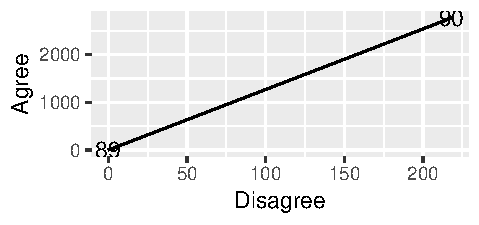
\includegraphics[width=\maxwidth]{figure/unnamed-chunk-2-1} 

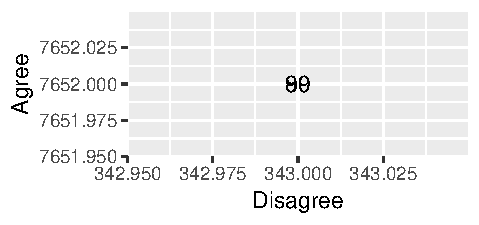
\includegraphics[width=\maxwidth]{figure/unnamed-chunk-2-2} 

\end{knitrout}
\caption{ROC for Gen1Housemates (left) and Gen2Siblings (right)}
\end{figure}

% latex table generated in R 3.5.3 by xtable 1.8-3 package
% Tue Mar 19 21:41:41 2019
\begin{table}[ht]
\centering
\begingroup\large
\begin{tabular}{lrrrrr}
  \hline
R & Implicit2004 & Implicit & Roster & Explicit & Eventual \\ 
  \hline
0 & - & 192 & 478 &  41 & 557 \\ 
  0.0625 & - & - & - &   2 &  45 \\ 
  0.125 &  76 & - &  96 & - &  96 \\ 
  0.25 &  43 & 180 & - & 273 & 297 \\ 
  0.375 & 310 & - & - &  37 &  15 \\ 
  0.5 & 1877 & 3515 & - & 3598 & 4006 \\ 
  0.75 &  32 & - & - & - &  11 \\ 
  1 & - & - & - & - &  11 \\ 
  - & 2964 & 1415 & 4728 & 1351 & 264 \\ 
   \hline
\end{tabular}
\endgroup
\caption{Counts for Gen1Housemates} 
\end{table}
% latex table generated in R 3.5.3 by xtable 1.8-3 package
% Tue Mar 19 21:41:41 2019
\begin{table}[ht]
\centering
\begingroup\large
\begin{tabular}{lrrrrr}
  \hline
R & Implicit2004 & Implicit & Roster & Explicit & Eventual \\ 
  \hline
- &   0 &   0 &   0 &   0 &   0 \\ 
   \hline
\end{tabular}
\endgroup
\caption{Counts for Gen1Housemates (Previous version of links)} 
\end{table}
% latex table generated in R 3.5.3 by xtable 1.8-3 package
% Tue Mar 19 21:41:41 2019
\begin{table}[ht]
\centering
\begingroup\large
\begin{tabular}{lrrrr}
  \hline
R & Implicit2004 & Implicit & Explicit & Eventual \\ 
  \hline
0.25 & 2221 & 3025 & 3003 & 3448 \\ 
  0.375 & 2663 & - & 267 & 622 \\ 
  0.5 & 5778 & 6741 & 5716 & 7004 \\ 
  0.75 & - &  13 & - &  13 \\ 
  1 &  36 &  27 &  23 &  27 \\ 
  - & 416 & 1308 & 2105 &   0 \\ 
   \hline
\end{tabular}
\endgroup
\caption{Counts for Gen2Siblings} 
\end{table}
% latex table generated in R 3.5.3 by xtable 1.8-3 package
% Tue Mar 19 21:41:41 2019
\begin{table}[ht]
\centering
\begingroup\large
\begin{tabular}{lrrrr}
  \hline
R & Implicit2004 & Implicit & Explicit & Eventual \\ 
  \hline
0.25 & 2221 & 3025 & 3003 & 3448 \\ 
  0.375 & 2663 & - & 267 & 622 \\ 
  0.5 & 5778 & 6741 & 5716 & 7004 \\ 
  0.75 & - &  13 & - &  13 \\ 
  1 &  36 &  27 &  23 &  27 \\ 
  - & 416 & 1308 & 2105 &   0 \\ 
   \hline
\end{tabular}
\endgroup
\caption{Counts for Gen2Siblings (Previous version of links)} 
\end{table}


% latex table generated in R 3.5.3 by xtable 1.8-3 package
% Tue Mar 19 21:41:41 2019
\begin{table}[ht]
\centering
\begin{tabular}{rrrrrr}
  \hline
Count & RImplicit2004 & RImplicit & RExplicit & RRoster & Delta \\ 
  \rowcolor{goodColor}  \hline
1444 & 0.500 & 0.500 & 0.500 & - & 1444 \\ 
   \rowcolor{goodColor} 1238 & - & 0.500 & 0.500 & - & 1238 \\ 
   \rowcolor{sosoColor} 501 & - & - & 0.500 & - & 501 \\ 
   \rowcolor{nullColor} 244 & - & - & - & - & 244 \\ 
  206 & 0.500 & 0.500 & - & - & 206 \\ 
  206 & - & 0.500 & - & - & 206 \\ 
   \rowcolor{sosoColor} 177 & 0.375 & - & 0.500 & - & 177 \\ 
   \rowcolor{sosoColor} 148 & - & - & 0.250 & - & 148 \\ 
  120 & - & 0.500 & - & 0.000 & 120 \\ 
   \rowcolor{nullColor} 99 & - & - & - & 0.000 & 99 \\ 
  76 & - & 0.000 & - & 0.000 & 76 \\ 
  72 & 0.500 & 0.500 & - & 0.000 & 72 \\ 
   \rowcolor{badColor} 59 & - & 0.500 & 0.250 & - & 59 \\ 
   \rowcolor{badColor} 50 & - & 0.250 & 0.500 & - & 50 \\ 
   \rowcolor{nullColor} 41 & 0.375 & - & - & - & 41 \\ 
   \rowcolor{goodColor} 39 & 0.375 & 0.500 & 0.500 & - & 39 \\ 
  32 & - & 0.000 & - & - & 32 \\ 
  32 & - & 0.250 & - & 0.000 & 32 \\ 
   \rowcolor{badColor} 31 & 0.500 & 0.250 & 0.500 & - & 31 \\ 
   \rowcolor{sosoColor} 27 & 0.500 & - & 0.500 & - & 27 \\ 
  22 & 0.125 & 0.500 & - & 0.125 & 22 \\ 
   \rowcolor{nullColor} 19 & 0.125 & - & - & 0.125 & 19 \\ 
   \rowcolor{badColor} 18 & 0.500 & 0.500 & 0.250 & - & 18 \\ 
   \rowcolor{sosoColor} 18 & - & - & 0.000 & - & 18 \\ 
   \rowcolor{sosoColor} 17 & 0.375 & - & 0.250 & - & 17 \\ 
  17 & - & 0.250 & - & - & 17 \\ 
  16 & 0.500 & 0.000 & - & 0.000 & 16 \\ 
   \rowcolor{nullColor} 15 & 0.500 & - & - & - & 15 \\ 
   \rowcolor{sosoColor} 15 & - & - & 0.375 & - & 15 \\ 
  14 & 0.500 & 0.250 & - & 0.000 & 14 \\ 
   \rowcolor{badColor} 14 & - & 0.000 & 0.500 & - & 14 \\ 
   \rowcolor{goodColor} 14 & - & 0.250 & 0.250 & - & 14 \\ 
   \rowcolor{sosoColor} 13 & 0.250 & - & 0.500 & - & 13 \\ 
   \rowcolor{goodColor} 12 & 0.750 & 0.500 & 0.500 & - & 12 \\ 
  11 & - & 0.500 & 0.375 & - & 11 \\ 
  11 & - & 0.500 & - & 0.125 & 11 \\ 
   \rowcolor{sosoColor} 10 & 0.125 & - & 0.500 & - & 10 \\ 
   \rowcolor{badColor} 10 & 0.500 & 0.000 & 0.500 & - & 10 \\ 
   \rowcolor{nullColor} 10 & - & - & - & 0.125 & 10 \\ 
  9 & - & 0.000 & - & 0.125 & 9 \\ 
   \rowcolor{badColor} 9 & - & 0.500 & 0.000 & - & 9 \\ 
   \rowcolor{nullColor} 8 & 0.250 & - & - & 0.000 & 8 \\ 
  7 & 0.125 & 0.250 & - & 0.125 & 7 \\ 
   \rowcolor{goodColor} 7 & 0.250 & 0.500 & 0.500 & - & 7 \\ 
   \rowcolor{nullColor} 7 & 0.250 & - & - & - & 7 \\ 
   \rowcolor{sosoColor} 7 & 0.750 & - & 0.500 & - & 7 \\ 
  6 & 0.500 & 0.250 & - & - & 6 \\ 
   \rowcolor{badColor} 5 & 0.375 & 0.000 & 0.500 & - & 5 \\ 
   \rowcolor{nullColor} 5 & 0.375 & - & - & 0.000 & 5 \\ 
  5 & 0.500 & 0.500 & 0.375 & - & 5 \\ 
   \rowcolor{nullColor} 5 & 0.750 & - & - & - & 5 \\ 
   \rowcolor{badColor} 5 & - & 0.000 & 0.250 & - & 5 \\ 
   \rowcolor{goodColor} 4 & 0.125 & 0.500 & 0.500 & - & 4 \\ 
  4 & 0.375 & 0.000 & - & 0.000 & 4 \\ 
  4 & 0.375 & 0.500 & - & 0.000 & 4 \\ 
  4 & 0.375 & 0.500 & - & - & 4 \\ 
   \rowcolor{sosoColor} 4 & 0.375 & - & 0.375 & - & 4 \\ 
  4 & 0.500 & 0.000 & - & - & 4 \\ 
  4 & - & 0.250 & - & 0.125 & 4 \\ 
   \rowcolor{nullColor} 3 & 0.125 & - & - & 0.000 & 3 \\ 
   \rowcolor{nullColor} 3 & 0.125 & - & - & - & 3 \\ 
   \rowcolor{goodColor} 3 & - & 0.000 & 0.000 & - & 3 \\ 
   \rowcolor{badColor} 3 & - & 0.500 & 0.250 & 0.000 & 3 \\ 
   \rowcolor{badColor} 2 & 0.125 & 0.500 & 0.000 & - & 2 \\ 
  2 & 0.250 & 0.500 & - & 0.000 & 2 \\ 
   \rowcolor{sosoColor} 2 & 0.250 & - & 0.250 & - & 2 \\ 
  2 & 0.375 & 0.000 & - & 0.125 & 2 \\ 
  2 & 0.375 & 0.000 & - & - & 2 \\ 
   \rowcolor{nullColor} 2 & 0.375 & - & - & 0.125 & 2 \\ 
   \rowcolor{badColor} 2 & 0.500 & 0.500 & 0.000 & - & 2 \\ 
  2 & 0.750 & 0.500 & - & - & 2 \\ 
   \rowcolor{nullColor} 2 & 0.750 & - & - & 0.000 & 2 \\ 
   \rowcolor{badColor} 2 & - & 0.000 & 0.500 & 0.000 & 2 \\ 
   \rowcolor{badColor} 2 & - & 0.500 & 0.000 & 0.000 & 2 \\ 
   \rowcolor{badColor} 2 & - & 0.500 & 0.000 & 0.125 & 2 \\ 
   \rowcolor{sosoColor} 2 & - & - & 0.250 & 0.000 & 2 \\ 
   \rowcolor{sosoColor} 2 & - & - & 0.500 & 0.000 & 2 \\ 
  1 & 0.125 & 0.000 & - & 0.125 & 1 \\ 
  1 & 0.125 & 0.000 & - & - & 1 \\ 
   \rowcolor{badColor} 1 & 0.125 & 0.500 & 0.000 & 0.125 & 1 \\ 
   \rowcolor{sosoColor} 1 & 0.125 & - & 0.000 & - & 1 \\ 
   \rowcolor{sosoColor} 1 & 0.125 & - & 0.250 & - & 1 \\ 
   \rowcolor{sosoColor} 1 & 0.125 & - & 0.500 & 0.125 & 1 \\ 
  1 & 0.250 & 0.000 & - & 0.000 & 1 \\ 
  1 & 0.250 & 0.000 & - & - & 1 \\ 
  1 & 0.250 & 0.500 & - & - & 1 \\ 
   \rowcolor{nullColor} 1 & 0.250 & - & - & 0.125 & 1 \\ 
   \rowcolor{goodColor} 1 & 0.375 & 0.000 & 0.000 & 0.000 & 1 \\ 
   \rowcolor{goodColor} 1 & 0.375 & 0.250 & 0.250 & - & 1 \\ 
  1 & 0.375 & 0.250 & - & - & 1 \\ 
   \rowcolor{goodColor} 1 & 0.375 & 0.500 & 0.500 & 0.000 & 1 \\ 
  1 & 0.500 & 0.250 & - & 0.125 & 1 \\ 
   \rowcolor{badColor} 1 & 0.500 & 0.500 & 0.062 & - & 1 \\ 
   \rowcolor{goodColor} 1 & 0.500 & 0.500 & 0.500 & 0.000 & 1 \\ 
  1 & 0.500 & 0.500 & - & 0.125 & 1 \\ 
   \rowcolor{sosoColor} 1 & 0.500 & - & 0.250 & - & 1 \\ 
   \rowcolor{sosoColor} 1 & 0.500 & - & 0.375 & - & 1 \\ 
   \rowcolor{nullColor} 1 & 0.500 & - & - & 0.000 & 1 \\ 
  1 & 0.750 & 0.000 & - & 0.000 & 1 \\ 
  1 & 0.750 & 0.000 & - & - & 1 \\ 
  1 & 0.750 & 0.250 & - & 0.000 & 1 \\ 
  1 & 0.750 & 0.500 & - & 0.000 & 1 \\ 
   \rowcolor{badColor} 1 & - & 0.000 & 0.375 & - & 1 \\ 
   \rowcolor{goodColor} 1 & - & 0.250 & 0.250 & 0.000 & 1 \\ 
   \rowcolor{badColor} 1 & - & 0.500 & 0.250 & 0.125 & 1 \\ 
   \rowcolor{goodColor} 1 & - & 0.500 & 0.500 & 0.000 & 1 \\ 
   \rowcolor{sosoColor} 1 & - & - & 0.062 & - & 1 \\ 
   \rowcolor{sosoColor} 1 & - & - & 0.500 & 0.125 & 1 \\ 
   \hline
\end{tabular}
\caption{Counts for Gen1Housemates} 
\end{table}
% latex table generated in R 3.5.3 by xtable 1.8-3 package
% Tue Mar 19 21:41:41 2019
\begin{table}[ht]
\centering
\begin{tabular}{rrrrrr}
  \hline
Count & RImplicit2004 & RImplicit & RExplicit & RRoster & Delta \\ 
  \rowcolor{goodColor}  \hline
4513 & 0.500 & 0.500 & 0.500 & - & 0 \\ 
   \rowcolor{goodColor} 1608 & 0.250 & 0.250 & 0.250 & - & 0 \\ 
  991 & 0.500 & 0.500 & - & - & 0 \\ 
   \rowcolor{goodColor} 546 & 0.375 & 0.250 & 0.250 & - & 0 \\ 
   \rowcolor{goodColor} 537 & 0.375 & 0.500 & 0.500 & - & 0 \\ 
   \rowcolor{nullColor} 468 & 0.375 & - & - & - & 0 \\ 
   \rowcolor{sosoColor} 370 & 0.375 & - & 0.250 & - & 0 \\ 
   \rowcolor{sosoColor} 255 & 0.375 & - & 0.500 & - & 0 \\ 
  196 & 0.250 & 0.250 & - & - & 0 \\ 
  166 & 0.375 & 0.500 & - & - & 0 \\ 
   \rowcolor{goodColor} 140 & - & 0.500 & 0.500 & - & 0 \\ 
  112 & 0.375 & 0.250 & - & - & 0 \\ 
   \rowcolor{goodColor} 109 & 0.500 & 0.250 & 0.250 & - & 0 \\ 
   \rowcolor{goodColor} 103 & - & 0.250 & 0.250 & - & 0 \\ 
  100 & 0.250 & 0.250 & 0.375 & - & 0 \\ 
   \rowcolor{badColor} 81 & 0.250 & 0.250 & 0.500 & - & 0 \\ 
   \rowcolor{badColor} 77 & 0.375 & 0.250 & 0.500 & - & 0 \\ 
   \rowcolor{goodColor} 73 & 0.250 & 0.500 & 0.500 & - & 0 \\ 
   \rowcolor{badColor} 72 & 0.500 & 0.500 & 0.250 & - & 0 \\ 
   \rowcolor{sosoColor} 66 & 0.250 & - & 0.250 & - & 0 \\ 
  62 & - & 0.500 & - & - & 0 \\ 
   \rowcolor{badColor} 50 & 0.375 & 0.500 & 0.250 & - & 0 \\ 
   \rowcolor{badColor} 44 & 0.250 & 0.500 & 0.250 & - & 0 \\ 
   \rowcolor{nullColor} 43 & - & - & - & - & 0 \\ 
  42 & 0.500 & 0.500 & 0.375 & - & 0 \\ 
   \rowcolor{sosoColor} 32 & 0.375 & - & 0.375 & - & 0 \\ 
   \rowcolor{sosoColor} 28 & - & - & 0.250 & - & 0 \\ 
  27 & 0.375 & 0.250 & 0.375 & - & 0 \\ 
  23 & 0.375 & 0.500 & 0.375 & - & 0 \\ 
   \rowcolor{goodColor} 22 & 1.000 & 1.000 & 1.000 & - & 0 \\ 
  19 & 0.500 & 0.250 & 0.375 & - & 0 \\ 
   \rowcolor{sosoColor} 17 & 0.250 & - & 0.500 & - & 0 \\ 
  17 & - & 0.250 & - & - & 0 \\ 
   \rowcolor{badColor} 13 & 0.500 & 0.250 & 0.500 & - & 0 \\ 
  12 & 1.000 & 0.750 & - & - & 0 \\ 
  11 & 0.250 & 0.500 & 0.375 & - & 0 \\ 
   \rowcolor{nullColor} 11 & 0.250 & - & - & - & 0 \\ 
  11 & 0.500 & 0.250 & - & - & 0 \\ 
  10 & 0.250 & 0.500 & - & - & 0 \\ 
   \rowcolor{sosoColor} 6 & - & - & 0.500 & - & 0 \\ 
   \rowcolor{sosoColor} 4 & 0.250 & - & 0.375 & - & 0 \\ 
  4 & - & 0.250 & 0.375 & - & 0 \\ 
   \rowcolor{badColor} 4 & - & 0.500 & 0.250 & - & 0 \\ 
   \rowcolor{sosoColor} 3 & 0.500 & - & 0.250 & - & 0 \\ 
  3 & - & 0.500 & 0.375 & - & 0 \\ 
   \rowcolor{sosoColor} 2 & 0.500 & - & 0.500 & - & 0 \\ 
  2 & 1.000 & 1.000 & - & - & 0 \\ 
   \rowcolor{badColor} 2 & - & 0.250 & 0.500 & - & 0 \\ 
   \rowcolor{sosoColor} 2 & - & - & 0.375 & - & 0 \\ 
   \rowcolor{goodColor} 1 & 0.500 & 1.000 & 1.000 & - & 0 \\ 
  1 & 0.500 & 1.000 & - & - & 0 \\ 
   \rowcolor{nullColor} 1 & 0.500 & - & - & - & 0 \\ 
  1 & - & 0.750 & - & - & 0 \\ 
  1 & - & 1.000 & - & - & 0 \\ 
   \hline
\end{tabular}
\caption{Counts for Gen2Siblings} 
\end{table}



\end{document}
